\documentclass[11pt]{beamer}

% \usetheme{CambridgeUS}
% \usecolortheme{dolphin}
\usepackage{amsmath}
\usepackage{amssymb}
\usepackage{amsfonts}

\usepackage{algorithm}
%\usepackage{algorithmic}
\usepackage{algorithmicx}
\usepackage{algpseudocode}

\usepackage{hyperref}
\usepackage[utf8]{inputenc}

\usepackage{graphicx}
\graphicspath{{./figures/}}
\usepackage[english]{babel}

\usepackage{url}
\usepackage{color}
\usepackage{xcolor}

\usepackage{tcolorbox}
\usepackage{minted}

\usefonttheme[onlymath]{serif}

\hypersetup{
  colorlinks,
  citecolor=green,
  linkcolor=black
}

\definecolor{darkgreen}{RGB}{0,128,0}
 
\hypersetup{
  colorlinks,
  citecolor=darkgreen,
  linkcolor=black
}

\usepackage{natbib}

\title{Decisions Trees, Random Forests and Ensemble Methods}
\author{Benoit Gaüzère}


\def\dbR{{\mathrm{I\hskip-2.2pt R}}}
\def\dbN{{\mathrm{I\hskip-2.2pt N}}}
\def\esp{{\mathrm{I\hskip-1.5pt E}}}
\def\pr{{\mathrm{I\hskip-2.2pt P}}}
\def\halam{{\widehat{\lambda}}}
\def\hasig{{\widehat{\sigma}}}
\def\hae{{\widehat{\varepsilon}}}
\def\tQ{{\widehat{Q}}}

\def\tR{{\widehat{R}}}
\def\halpha{{\widehat{\alpha}}}
\def\haa{{\widehat{a}}}
\def\ha{{\widehat{a}}}
\def\he{{\widehat{\varepsilon}}}
\def\hb{{\widehat{b}}}
\def\hab{{\widehat{b}}}
\def\haE{{\widehat{E}}}
\def\hsigma{{\widehat{\sigma}}}
\def\hay{{z}}
\def\baR{{\overline{R}}}
\def\baE{{\overline{E}}}
\def\baX{{\overline{X}}}
\def\bax{{\overline{x}}}
\def\baY{{\overline{Y}}}
\def\bay{{\overline{y}}}
\def\barY{{\overline{Y}}}
\def\mx{{\overline{x}}}
\def\my{{\overline{y}}}
\def\lamMV{{\widehat{\lambda}_{MV}}}
\def\lamef{{\widehat{\lambda}_{e}}}

%\def\dbC{{\mathrm{I\hskip-5.4pt C}}}
\def\dbC{{\mathds{C}}}
\def\un{{\mathds{1}}}
\def\a{{\mathrm{a}}}
\def\b{{\mathrm{b}}}
\def\bc{{\mathrm{c}}}
\def\d{{\boldsymbol{d}}}
\def\e{{\mathrm{e}}}
\def\m{{\mathrm{m}}}
\def\n{{\mathrm{n}}}
\def\p{{\mathrm{p}}}
\def\r{{\mathrm{r}}}
\def\s{{\mathrm{s}}}
\def\u{{\mathrm{u}}}
\def\v{{\mathrm{v}}}
\def\ones{{\boldsymbol{\mathbb{1}}}}
\def\w{{\boldsymbol{w}}}
\def\x{{\mathbf{x}}}
\def\X{{\boldsymbol{X}}}
\def\y{{\boldsymbol{y}}}
\def\z{{\boldsymbol{z}}}
\def\tx{{\widetilde{x}}}
\def\bPhi{{\mathrm{\Phi}}}
\def \habeta{{\widetilde{\beta}}}
\def\Cmat{{\boldsymbol{C}}}

\def\tL{{\widetilde{L}}}
\def\tF{{\widetilde{F}}}
\def\tM{{\widetilde{M}}}
\def\tH{{\widetilde{H}}}
\def\tD{{\widetilde{D}}}
\def\tU{{\widetilde{U}}}
\def\vh{{\bar{v}^\top}}
\def\det{{\mbox{det}}}
\def\atimes{{\alert{\times}}}

\def\clO{{\mathcal{O}}}
\def\clA{{\mathcal{A}}}
\def\clB{{\mathcal{B}}}
\def\clD{{\mathcal{D}}}
\def\clL{{\mathcal{L}}}
\def\clN{{\mathcal{N}}}
\def\clH{{\mathcal{H}}}
\def\clT{{\mathcal{T}}}
\def\clY{\mathcal{Y}}
\def\fl{{\mbox{fl}}}

%\input{notation}

%%%%%%%%%%%%%%%%%%%%%%%%%%%%%%%%%%%%%%%%%%%%%%%%%%%%%%%%%%
\def\dbC{{\mathrm{I\hskip-4.7pt C}}}
\def\dbR{{\mathrm{I\hskip-2.2pt R}}}
\def\un{{\mathrm{I\hskip-5.9pt 1}}}
\def\dbN{{\mathrm{I\hskip-2.2pt N}}}
\def\esp{{\mathrm{I\hskip-1.5pt E}}}
\def\pr{{\mathrm{I\hskip-2.2pt P}}}
\def\hpr{\widehat{\mathrm{I\hskip-2.2pt P}}}
%\def\balpha{{\mathbf{\alpha}}}
\def\a{{\mathbf{a}}}
\def\b{{\mathbf{b}}}
\def\bc{{\mathbf{c}}}
%\def\d{{\mathbf{d}}}
\def\e{{\mathbf{e}}}
\def\f{{\mathbf{f}}}
\def\g{{\mathbf{g}}}
\def\h{{\mathbf{h}}}
\def\p{{\mathbf{p}}}
\def\q{{\mathbf{q}}}
\def\u{{\mathbf{u}}}
\def\v{{\mathbf{v}}}
%def\x{{\mathbf{x}}}
\def\xb{{\overline{x}}}
\def\yb{{\overline{y}}}
%\def\w{{\mathbf{w}}}
\def\haF{{\widehat{F}}}
\def\hap{{\widehat{p}}}
\def\R{\mathbb{R}}
\def\P{\mathbb{P}}
\def\E{\mathbb{E}}
\def\bX{\mathbb{X}}
\def\haF{{\widehat{F}}}
\def\haf{{\widehat{f}}}
\def\ham{{\widehat{m}}}
\def\haM{{\widehat{M}}}
\def\hamu{{\widehat{\mu}}}
\def\hasigma{{\widehat{\sigma}}}
\def\hap{{\widehat{\pr}}}
\def\haphi{{\widehat{\phi}}}
\def\haS{{\widehat{S}}}
\def\has{{\widehat{s}}}
\def\haQ{{\widehat{Q}}}
\def\hamc{{\widehat{mc}}}
\def\barX{{\bar{X}}}
\def\barx{{\bar{x}}}
\def\bary{{\bar{y}}}
\def\haPr{{\widehat{\mathrm{I\hskip-2.2pt P}}}}
\def\hap{{\widehat{p}}}
\def\bmu{{\boldsymbol{\mu}}}
\def\point{{\mbox{\tiny\textbullet}}}

%%%%%%%%%%%%%%%%%%%%%%%%%%%%%%%%%%%%%%%%%%%%%%%%%%%%%%%%%%%%%%%%%%%%%%%%%%%%%%%%%%%%%%%%%%%%%%%%%%%%%%%%%%%%%%%%%%%%%%%%%%%%
%%%%%%%%%%%%%%%%%%%%%%%%%%%%%%%%%%%%%%%%%%%%%%%%%%%%%%%%%%%%%%%%%%%%%%%%%%%%%%%%%%%%%%%%%%%%%%%%%%%%%%%%%%%%%%%%%%%%%%%%%%%%

\def\dbR{{\mathrm{I\hskip-2.2pt R}}}
\def\dbN{{\mathrm{I\hskip-2.2pt N}}}
\def\esp{{\mathrm{I\hskip-1.5pt E}}}
\def\pr{{\mathrm{I\hskip-2.2pt P}}}
\def\halam{{\widehat{\lambda}}}
\def\hasig{{\widehat{\sigma}}}
\def\tQ{{\widehat{Q}}}

\def\tR{{\widehat{R}}}
\def\haa{{\widehat{a}}}
\def\hab{{\widehat{b}}}
\def\haE{{\widehat{E}}}
\def\baR{{\overline{R}}}
\def\baE{{\overline{E}}}
\def\baX{{\overline{X}}}
\def\baY{{\overline{Y}}}
\def\lamMV{{\widehat{\lambda}_{MV}}}
\def\lamef{{\widehat{\lambda}_{e}}}
\def\k{{\mathnormal{k}}}
\def\f{{\mathnormal{f}}}
\def\g{{\mathnormal{g}}}
\def\datax{{\mathnormal{x}}}
\def\K{{\mathbf{K}}}
\def\G{{\mathbf{G}}}

%\def\dbC{{\mathrm{I\hskip-5.4pt C}}}
\def\dbC{{\mathds{C}}}
\def\un{{\mathds{1}}}
\def\a{{\mathbf{a}}}
\def\b{{\mathbf{b}}}
\def\c{{\mathbf{c}}}
%\def\d{{\mathbf{d}}}
\def\e{{\mathbf{e}}}
\def\m{{\mathbf{m}}}
\def\p{{\mathbf{p}}}
\def\r{{\mathbf{r}}}
\def\u{{\mathbf{u}}}
\def\v{{\mathbf{v}}}
%\def\w{{\mathbf{w}}}

\def\Un{{\mathrm{{1\hskip-2.6pt I}}}}

\def\dist{{d_m}}

\def\t{{\mathbf{t}}}
\def\s{{\mathbf{s}}}
%def\x{{\mathbf{x}}}

\def\tx{{\widetilde{x}}}
\def\tL{{\widetilde{L}}}
\def\tF{{\widetilde{F}}}
\def\tM{{\widetilde{M}}}
\def\tH{{\widetilde{H}}}
\def\ttau{{\widetilde{\tau}}}
\def\tD{{\widetilde{D}}}
\def\tU{{\widetilde{U}}}
\def\vh{{\bar{v}^\top}}
\def\det{{\mbox{det}}}
\def\atimes{{\alert{\times}}}

\def\balpha{{\boldsymbol\alpha}}
\def\bbeta{{\boldsymbol\beta}}
\def\clO{{\mathcal{O}}}
\def\clA{{\mathcal{A}}}
\def\clL{{\mathcal{L}}}
\def\clQ{{\mathcal{Q}}}
\def\clD{{\mathcal{D}}}
\def\clX{{\mathcal{X}}}
\def\clH{{\mathcal{H}}}
\def\clY{{\mathcal{Y}}}
\def\clP{{\mathcal{P}}}
\def\clS{{\mathcal{S}}}
\def\bfX{{\mathbf{X}}}
\def\bfB{{\mathbf{B}}}
\def\bfA{{\mathbf{A}}}

\def\bfI{{\mathbf{I}}}
\def\fl{{\mbox{fl}}}

\def\R{{\mathbb{N}}}
\def\R{{\mathbb{R}}}
\def\0{{\mathbf{0}}}
\def\1{{\mathbb{1}}}
\DeclareMathOperator*{\argmin}{argmin}
\DeclareMathOperator*{\argmax}{argmax} 
\DeclareMathOperator*{\mymin}{min}
\DeclareMathOperator*{\mymax}{max}
\RequirePackage{bbold}
\RequirePackage{kvoptions}

\newcommand{\complex}[1]{\mbox{$\mathcal{O}(#1)$}}
\newcommand{\cluster}[1]{\mbox{$\mathcal{C}_{#1}$}}


\def\T{{\mathsf{T}}}
\newcommand\dangersign[1][2ex]{%
  \renewcommand\stacktype{L}%
  \scaleto{\stackon[1.3pt]{\color{red}$\triangle$}{\tiny !}}{#1}%
}
\renewcommand{\vec}[1]{\mathbf{#1}}


\DeclareMathOperator*{\triinf}{\tt tri\_inf}
\DeclareMathOperator*{\diag}{\tt diag}

\newcommand{\Perm}[2]{P_{#1 \leftrightarrow #2}}
\DeclareMathOperator*{\triinfunit}{\tt tri\_inf\_unit}
\DeclareMathOperator*{\triangularise}{\tt factorisation\_LU}
\DeclareMathOperator*{\factopalu}{\tt factorisation\_PALU}
\DeclareMathOperator*{\factoldm}{\tt factorisation\_LDM}
\DeclareMathOperator*{\factoldl}{\tt factorisation\_LDL}
\DeclareMathOperator*{\factochol}{\tt Cholesky}
\DeclareMathOperator*{\factocholrec}{\tt Cholesky\_Rec}
\DeclareMathOperator*{\factocholinc}{\tt Cholesky\_Incr}
\DeclareMathOperator*{\trisup}{\tt tri\_sup}
\DeclareMathOperator*{\tfgauss}{\tt Tf\_Gauss}
\DeclareMathOperator*{\gausselim}{\tt Gauss\_Elimination}
\DeclareMathOperator*{\mettreajour}{\tt mettre\_a\_jour}
\DeclareMathOperator*{\triu}{\tt triu}
\DeclareMathOperator*{\assign}{\leftarrow}
\DeclareMathOperator*{\resolve}{\tt resoud}
\DeclareMathOperator*{\swap}{\leftrightarrow}
\newenvironment{rcases} 
        {\left.\begin{aligned}}
         {\end{aligned}\hspace{0.5cm}\right\rbrace}

% \renewenvironment{definition}[1]
% {
%   \begin{mdframed}[backgroundcolor=blue]
%     \textbf{Définition : #1}\\
%     \setlength{\alglength}{.95\linewidth} \begin{minipage}[t]{\alglength}
% }{        \end{minipage}
%     % \end{algorithmfloat}
%   \end{mdframed}
% }
\renewcommand{\emph}[1]{{\color{blue} #1}}
\renewenvironment{definition}[1][]{%                                                                         
  \ifstrempty{#1}%                                                                                   
  {\mdfsetup{%                                                                                       
    frametitle={%                                                                                    
      \tikz[baseline=(current bounding box.east),outer sep=0pt]                                     
       \node[anchor=east,rectangle,fill=blue!20]                                                    
        {\strut Définition};}}                                                                 
  }%                                                                                                 
  {\mdfsetup{%                                                                                       
      frametitle={%                                                                                   
        \tikz[baseline=(current bounding box.east),outer sep=0pt]                                     
        \node[anchor=east,rectangle,fill=blue!20]                                                    
        {\strut Définition~:~#1};}}%                                                            
  }%                                                                                                
  \mdfsetup{innertopmargin=10pt,linecolor=blue!20,%                                                 
    linewidth=2pt,topline=true,                                                             
    frametitleaboveskip=\dimexpr-\ht\strutbox\relax,}                                       
  \begin{mdframed}[]\relax%                                                                         
  }{\end{mdframed}}                                                                                 

\renewenvironment{lemma}[1][]{%                                                                         
  \ifstrempty{#1}%                                                                                   
  {\mdfsetup{%                                                                                       
    frametitle={%                                                                                    
      \tikz[baseline=(current bounding box.east),outer sep=0pt]                                     
       \node[anchor=east,rectangle,fill=green!10]                                                    
        {\strut Lemme};}}                                                                 
  }%                                                                                                 
  {\mdfsetup{%                                                                                       
      frametitle={%                                                                                   
        \tikz[baseline=(current bounding box.east),outer sep=0pt]                                     
        \node[anchor=east,rectangle,fill=green!10]                                                    
        {\strut Lemme~:~#1};}}%                                                            
  }%                                                                                                
  \mdfsetup{innertopmargin=10pt,linecolor=green!10,%                                                 
    linewidth=2pt,topline=true,                                                             
    frametitleaboveskip=\dimexpr-\ht\strutbox\relax,}                                       
  \begin{mdframed}[]\relax%                                                                         
  }{\end{mdframed}}                                                                                 

\renewenvironment{theorem}[1][]{%                                                                         
  \ifstrempty{#1}%                                                                                   
  {\mdfsetup{%                                                                                       
    frametitle={%                                                                                    
      \tikz[baseline=(current bounding box.east),outer sep=0pt]                                     
       \node[anchor=east,rectangle,fill=green!50]                                                    
        {\strut Théorème};}}                                                                 
  }%                                                                                                 
  {\mdfsetup{%                                                                                       
      frametitle={%                                                                                   
        \tikz[baseline=(current bounding box.east),outer sep=0pt]                                     
        \node[anchor=east,rectangle,fill=green!50]                                                    
        {\strut Théorème~:~#1};}}%                                                            
  }%                                                                                                
  \mdfsetup{innertopmargin=10pt,linecolor=green!50,%                                                 
    linewidth=2pt,topline=true,                                                             
    frametitleaboveskip=\dimexpr-\ht\strutbox\relax,}                                       
  \begin{mdframed}[]\relax%                                                                         
  }{\end{mdframed}}                                                                                 

\renewenvironment{corollary}[1][]{%                                                                         
  \ifstrempty{#1}%                                                                                   
  {\mdfsetup{%                                                                                       
    frametitle={%                                                                                    
      \tikz[baseline=(current bounding box.east),outer sep=0pt]                                     
       \node[anchor=east,rectangle,fill=green!25]                                                    
        {\strut Corollaire};}}                                                                 
  }%                                                                                                 
  {\mdfsetup{%                                                                                       
      frametitle={%                                                                                   
        \tikz[baseline=(current bounding box.east),outer sep=0pt]                                     
        \node[anchor=east,rectangle,fill=green!25]                                                    
        {\strut Corollaire~:~#1};}}%                                                            
  }%                                                                                                
  \mdfsetup{innertopmargin=10pt,linecolor=green!25,%                                                 
    linewidth=2pt,topline=true,                                                             
    frametitleaboveskip=\dimexpr-\ht\strutbox\relax,}                                       
  \begin{mdframed}[]\relax%                                                                         
  }{\end{mdframed}}                                                                                 


% \newenvironment{theo}[1][]{%
%   \ifstrempty{#1}{
%     \mdfsetup{% 
%       frametitle=%
%       \tikz[baseline =(current bounding box.east)]
%       \node[anchor=east,rectangle,fill=blue!20]
%       {\strut ~Définition};}}
%   {
%     \mdfsetup{%
%       frametitle={%
%         \tikz[baseline=(current bounding box.east)]
%         % \node[anchor=east,rectangle,fill=blue!20]
%         {\strut Définition:~#1};}}%
%   }%
%   \mdfsetup{innertopmargin=10pt,linecolor=blue!20,%
%     linewidth=2pt,topline=true,
%     frametitleaboveskip=\dimexpr-\ht\strutbox\relax,}
%   \begin{mdframed}[]\relax  % 
%   }{
%   \end{mdframed}
% }

\setbeamertemplate{footline}[frame number]
\setbeamertemplate{navigation symbols}{}

\addto\captionsfrench{%
  \renewcommand{\figurename}{Fig.}
}

\def\danger{
\includegraphics[width=0.6cm]{danger}}
\def\bigdanger{
\includegraphics[width=1cm]{danger}}
\def\smalldanger{
\includegraphics[width=.4cm]{danger}}

\def\pn{{\mathnormal{n}}}
\def\pz{{\mathnormal{z}}}
\def\pp{{\mathnormal{p}}}

\def\px{{\mathnormal{x}}}
\def\ps{{\mathnormal{s}}}
\def\pt{{\mathnormal{t}}}

\renewcommand\diag[4]{%
  \multicolumn{1}{p{#2}|}{\hskip-\tabcolsep
  $\vcenter{\begin{tikzpicture}[baseline=0,anchor=south west,inner sep=#1]
  \path[use as bounding box] (0,0) rectangle (#2+2\tabcolsep,\baselineskip);
  \node[minimum width={#2+2\tabcolsep-\pgflinewidth},
        minimum  height=\baselineskip+\extrarowheight-\pgflinewidth] (box) {};
  \draw[line cap=round] (box.north west) -- (box.south east);
  \node[anchor=south west] at (box.south west) {#3};
  \node[anchor=north east] at (box.north east) {#4};
 \end{tikzpicture}}$\hskip-\tabcolsep}}

\newcommand{\blue}[1]{\textcolor{blue}{#1}}
\newcommand{\green}[1]{\textcolor{darkgreen}{#1}}
\newcommand{\arrow}{
   \includegraphics[width=0.5cm]{fleche}
}

\newcommand{\doublearrow}{
  
\includegraphics[width=0.5cm]{flechedouble}
}

\newcommand*{\itemperso}{\includegraphics[width=0.8em]{item}}
\newcommand{\xvec}{\mathbf{x}}
\newcommand{\xiivec}{\mathbf{x_i}}
\newcommand{\xjjvec}{\mathbf{x_j}}
\newcommand{\xpvec}{\mathbf{x'}}
\newcommand{\wvec}{\mathbf{w}}
\newcommand{\betavec}{\mathbf{\beta}}
\newcommand{\alphavec}{\mathbf{\alpha}}
\newcommand{\xivec}{\mathbf{\xi}}


\renewcommand{\complex}[1]{\mbox{$\mathcal{O}(#1)$}}
%\DeclareMathOperator{\dist}{d}
\DeclareMathOperator{\sub}{\# sub}
\DeclareMathOperator{\code}{code}
\DeclareMathOperator{\struct}{struct}
\DeclareMathOperator{\myminimize}{minimize}
\DeclareMathOperator{\mymaximize}{maximize}
\newcommand{\minimiser}[1]{\underset{#1}{\myminimize}}
\newcommand{\maximiser}[1]{\underset{#1}{\mymaximize}}
%\DeclareMathOperator{\mymin}{min}
%\DeclareMathOperator{\mymax}{max}
\newcommand{\vecmath}[1]{\mathbf{#1}}

\newcommand*{\itemplus}{
\includegraphics[width=0.8em]{plus}}
\newcommand*{\itemdanger}{\includegraphics[width=1em]{warning}}
\newcommand*{\itemmoins}{
\includegraphics[width=0.8em]{moins}}

\renewcommand{\H}{\ensuremath{\mathcal{H}}}

\newcommand{\myinf}{
  
\includegraphics[width=0.4cm]{inf}
}
\newcommand{\myinfbar}{
  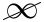
\includegraphics[width=0.4cm]{infbar}
}

\newcommand{\beginbackup}{
   \newcounter{framenumbervorappendix}
   \setcounter{framenumbervorappendix}{\value{framenumber}}
}
\newcommand{\backupend}{
   \addtocounter{framenumbervorappendix}{-\value{framenumber}}
   \addtocounter{framenumber}{\value{framenumbervorappendix}} 
}

\usefonttheme[onlymath]{serif}


\institute{INSA Rouen Normandie - Laboratoire LITIS}

% =================================================================================
\begin{document}
\maketitle

% =================================================================================

\begin{frame}{Outline}
  \tableofcontents
\end{frame}

\section{Decision Tree}
\begin{frame}{Introduction to Decision Trees}
    \begin{itemize}
        \item Supervised learning for classification and regression.
        \item Simple to understand and interpret.
        \item Recursive algorithm to construct the decision trees
    \end{itemize}

\centering{ 

\includegraphics[width=.7\textwidth]{flowchart}
    }
    
\end{frame}



\begin{frame}
  \frametitle{Decision Tree}
  \begin{block}{Principle}
    Learn decision rules to separate the data.
    \begin{center}
      \only<1>{
        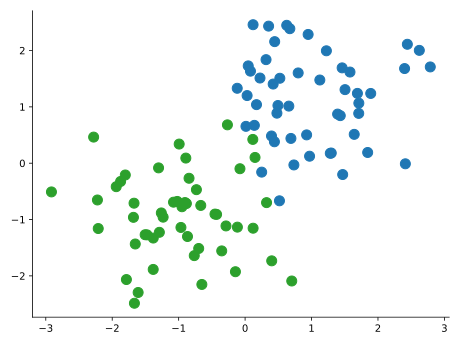
\includegraphics[width=.75\textwidth]{decision_tree_data}
      }
      \only<2>{
        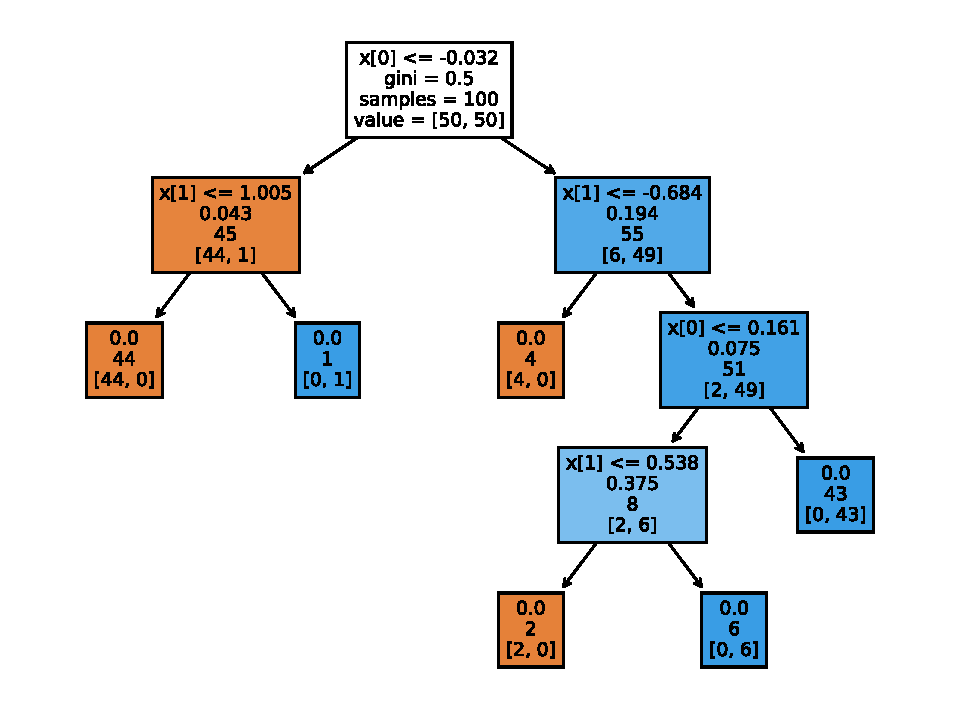
\includegraphics[width=.75\textwidth]{decision_tree_tree}
      }
      \only<3>{
        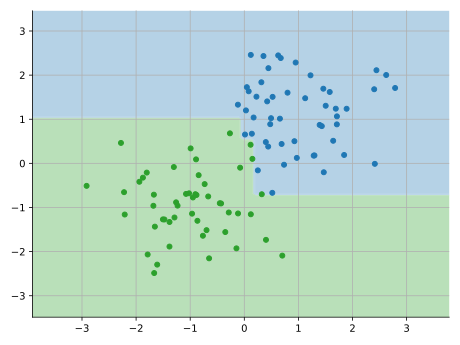
\includegraphics[width=.75\textwidth]{decision_tree_boundary}
        }
    \end{center}
    
  \end{block}

  
\end{frame}



% =================================================================================
\subsection{Decision Tree Algorithm}
% =================================================================================

\begin{frame}
  \frametitle{How to learn Decision Trees ? }
  \begin{block}{Split Data}
    \begin{enumerate}
    \item Choose a feature $f$
    \item Compute a threshold $t_f$
    \end{enumerate}
    \pause
  \end{block}
  \begin{center}
    \emph{How to determine $t_f$ ? (and $f$) }
  \end{center}
  \pause
  \begin{block}{Maximize Information Gain}
    $$
    IG(D_p,f)  = I(D_p) - \frac{N_l}{N_p} I(D_l) - \frac{N_r}{N_p} I(D_r)
    $$

    with:
    \begin{itemize}
    \item $I$ : measure of impurity
    \item $D_p$, $D_l$ and $D_r$ the datasets corresponding to parent, left node and right node.
    \end{itemize}

  \end{block}
\end{frame}

\begin{frame}[allowframebreaks]
  \frametitle{Impurity measures}
  \framesubtitle{To minimize !}
  \begin{block}{Entropy}
    %2 classes
    $$
    I_e(p)= - p * log_2(p) - (1-p) * log_2(1-p)
    $$
    with $p$ characterizing the probability for a sample to belong to one class
    in a given node ($P(C_k | D)$).
    \begin{center}
   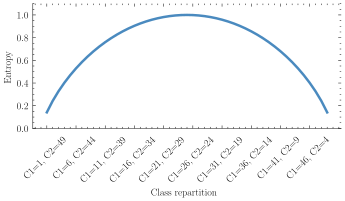
\includegraphics[width=.6\textwidth]{entropy}
   \end{center}
 \end{block}
%\framebreak
  %Very similar to entropy.
    % minimize the misclassification error
    
  \begin{block}{Gini Impurity}
    $$
    I_G(p) = \sum_{i=1}^c p_i * (1-p_i) = 1 - \sum_{i=1}^c p_i^2
    $$
    for $c=2, I_G(p) = 1 - p^2 - (1-p)^2$. 
    \begin{center}
    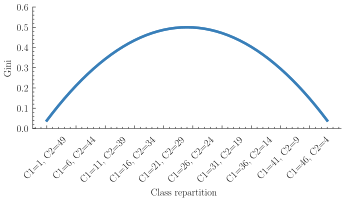
\includegraphics[width=.6\textwidth]{gini}
  \end{center}
\end{block}

  \begin{block}{Classification error}
    $$I_E(p) = 1 - \max_{i \in 1 \dots c} {p_i}$$
    Less sensitive to good repartition.
    \begin{center}
    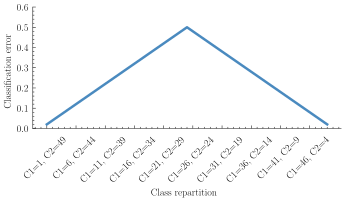
\includegraphics[width=.6\textwidth]{ce}
  \end{center}
  \end{block}

\end{frame}

\begin{frame}
  \frametitle{Differences between impurity}
  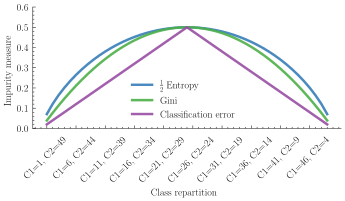
\includegraphics[width=\textwidth]{impurity_measures}
\end{frame}

\begin{frame}
  \frametitle{The CART algorithm}

  \begin{algorithmic}
    \Function{split\_recur}{$D$}
      \If{not a leaf}
       \State $\theta^\star = \argmax_\theta IG(D,\theta)$
       \State $D_l,D_r = \textrm{partition}(D,\theta^\star)$
       \State $\textsc{split\_recur}(D_l)$
       \State $\textsc{split\_recur}(D_r)$
       \EndIf
       \EndFunction
 \end{algorithmic}
 
  \begin{itemize}
  \item with $\theta = (f,tf)$
  \item Recursively select the best split which maximize the IG
  \item When does it stop ?
    \pause
    \begin{itemize}
    \item Only one class in $D$
    \item Max depth reach
    \item Min number of samples $D$ reached
    \end{itemize}
  \end{itemize}
%%   p182, aurélien géron
%%   \url{https://scikit-learn.org/stable/modules/tree.html#mathematical-formulation}
\end{frame}

\begin{frame}
    \frametitle{Hyperparameters of Decision Tree}
    \begin{block}{Maximum depth}
    Specify the maximal depth of the tree. An higher depth will make dedicate
    categories, but prone to overfit.
    \end{block}
    \vfill
    \begin{block}{Min number of splits}
      Same action as previous one. 
    \end{block}
    \begin{center}

    $\to$ Both are used to terminate the recursive operation
    \end{center}
    
\end{frame}


\begin{frame}[fragile]
  \frametitle{Building a decision tree - the code}
  
  \begin{minted}
    [
      frame=lines,
      framesep=2mm,
      baselinestretch=1.2,
      fontsize=\footnotesize,
      linenos
    ]
    {python}
    from sklearn.tree import DecisionTreeClassifier
    max_depth = 10
    criterion = 'gini'
    clf = DecisionTreeClassifier(max_depth=max_depth,
    criterion=criterion)
    clf = clf.fit(X, y)
    ypred = clf.predict(X)
  \end{minted}

  \begin{itemize}
  \item User guide for hyperparameters  :
    \href{https://scikit-learn.org/stable/modules/tree.html#tips-on-practical-use}{link}
  \item $\Rightarrow$ Notebook
    %% \item Exists for regression problems
  \item the
    \href{https://scikit-learn.org/stable/modules/generated/sklearn.tree.DecisionTreeClassifier.html#sklearn.tree.DecisionTreeClassifier}{documentation}
    %% \item la
    %%   \href{https://scikit-learn.org/stable/modules/generated/sklearn.ensemble.RandomForestRegressor.html#sklearn.ensemble.RandomForestRegressor}{doc
    %%     regressor}
  \end{itemize}

\end{frame}


\begin{frame}
  \frametitle{Limitations}
  \begin{itemize}
  \item Simple yet effective algorithm
  \item Prone to overfitting \\
    $\to$ one leaf $\Leftrightarrow$ one sample
  \end{itemize}
  \pause
  \begin{center}
  
\includegraphics[width=.7\textwidth]{transition_decision_tree}
  \end{center}
\end{frame}

\section{Ensemble Methods}
\begin{frame}
  \frametitle{Ensemble Methods}
  \begin{block}{Idea}
    United we stand
    \begin{center}

    
\includegraphics[width=.7\textwidth]{ensemble_principle}
    \end{center}
  \end{block}
  \begin{block}{How to combine them ?}
    
  \begin{itemize}
  \item Majority voting,  Bagging and  Boosting
  \end{itemize}
    \end{block}

\end{frame}


\subsection{Random Forests}
\begin{frame}[plain]

  \begin{center}
    \Huge{Random Forests}
    \end{center}
  
\end{frame}


\begin{frame}
    \frametitle{Random Forests}
    \begin{block}{Principle}
      \begin{itemize}
      \item Combine many decision trees to learn complex functions
      \item Ensemble methods, majority voting 
      \item Bagging \cite{breiman1996bagging}
      \end{itemize}
  
      \begin{center}
        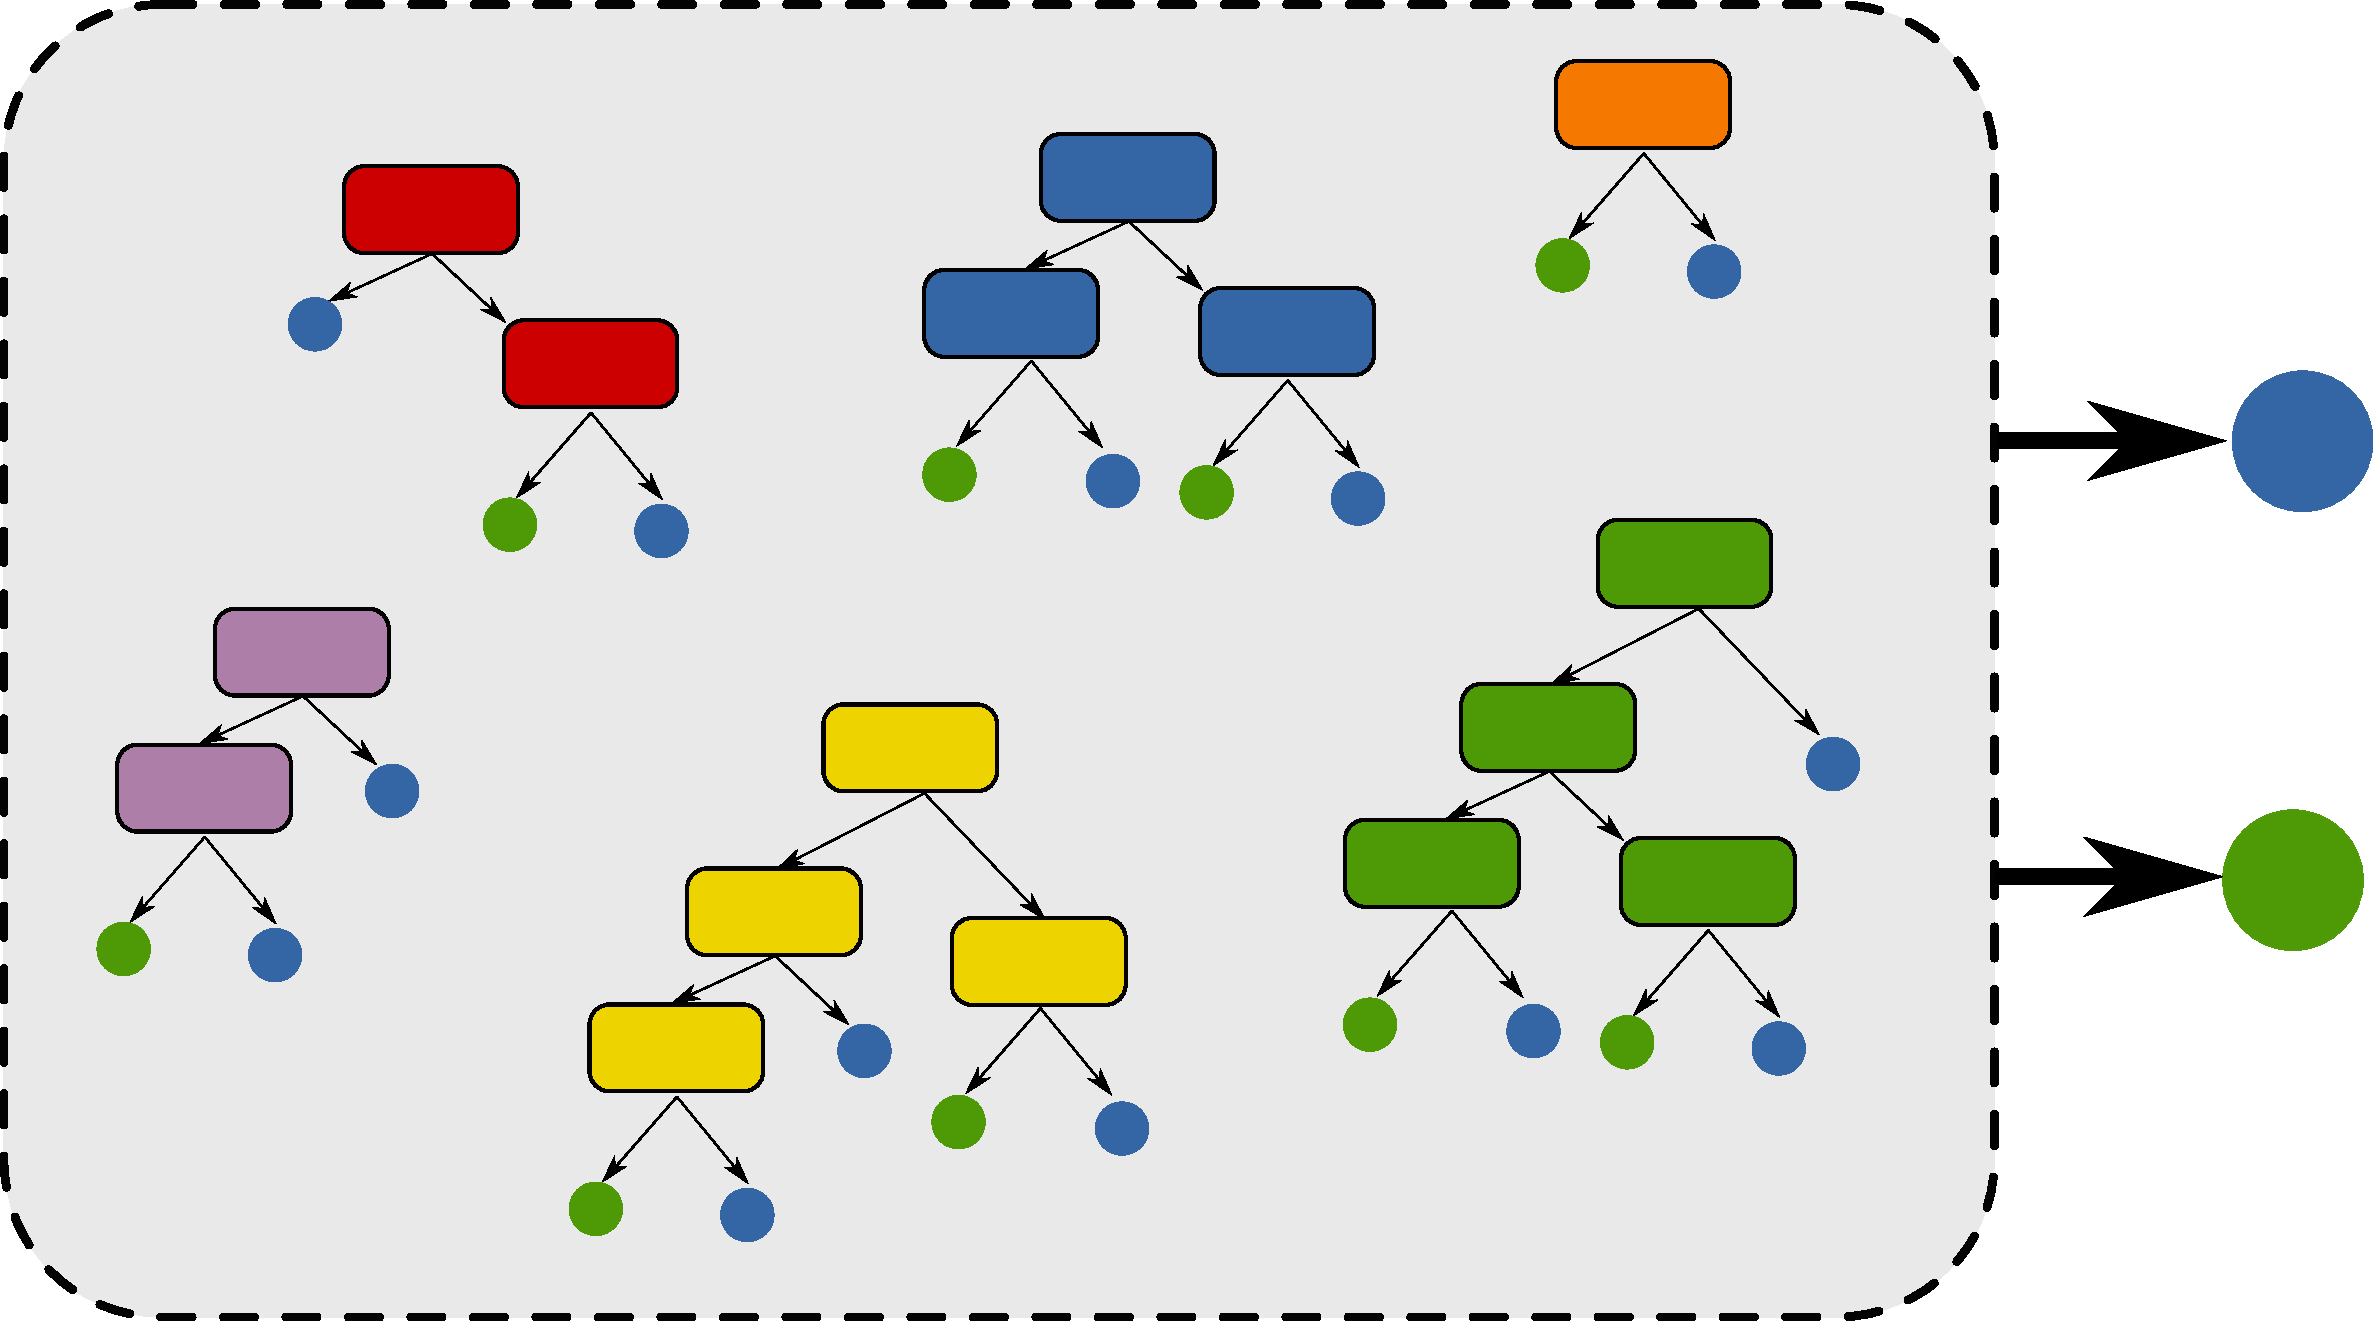
\includegraphics[width=.7\textwidth]{random_forests}
      \end{center}
    \end{block}
   
  \end{frame}


\begin{frame}
  \frametitle{Algorithm summarization}
  \begin{enumerate}
  \item Randomly choose $n$ examples (bootstrap)
  \item Build a decision tree from the bootstrap
    \begin{enumerate}
    \item Randomly select $d$ features
    \item Split according to best pair feature/threshold
    \end{enumerate}
  \item Repeat $k$ times
  \item Aggregate decision by majority vote or average probability 
  \end{enumerate}
\end{frame}

\begin{frame}[fragile]
  \frametitle{Random Forests Hyperparameters}

  \begin{block}{Number of trees}
    Adjust the number of trees composing the forests
    \begin{itemize}
    \item low number : fast to compute, but less accurate
    \item high number : slower to compute, but more accurate up to some number
    \end{itemize}
  \end{block}

  \begin{block}{Number of features}
    Determine the number of features to be used when splitting the data
    \begin{itemize}
    \item See the guidelines of \verb|scikit-learn|
    \end{itemize}
  \end{block}

  \begin{block}{Tree depth}
    Specify the maximal depth of tree. An higher depth will make dedicate
    categories, but less generalizable.
  \end{block}
\end{frame}

\begin{frame}[fragile]
  \frametitle{Random Forests : the code !}
  
  \begin{minted}
[
frame=lines,
framesep=2mm,
baselinestretch=1.2,
fontsize=\footnotesize,
linenos
]
{python}
from sklearn.ensemble import RandomForestClassifier
n_estimators = 20 # the number of trees in the forest
max_depth = None # expand as you can
max_features = "sqrt" # RTFM
clf = RandomForestClassifier(n_estimators=n_estimators,
                             max_depth=max_depth,
                             max_features=max_features)
clf.fit(X,y)
ypred = clf.predict(X)
\end{minted}

\begin{itemize}
\item User guide for hyperparameters  :
  \href{https://scikit-learn.org/stable/modules/ensemble.html#forest}{link}
  
\item $\Rightarrow$ Notebook
%% \item Exists for regression problems
  \item the
  \href{https://scikit-learn.org/stable/modules/generated/sklearn.ensemble.RandomForestClassifier.html#sklearn.ensemble.RandomForestClassifier}{documentation}
%% \item la
%%   \href{https://scikit-learn.org/stable/modules/generated/sklearn.ensemble.RandomForestRegressor.html#sklearn.ensemble.RandomForestRegressor}{doc
%%     regressor}
\end{itemize}

\end{frame}

\section{Gradient Boosting}
\begin{frame}[plain]

  \begin{center}
    \Huge{Boosting}
    \end{center}
  
\end{frame}



\begin{frame}
  \frametitle{Boosting}
  \cite{schapire1990strength}

  \begin{block}{Principle}
    \begin{itemize}
    \item Weak learners, just better than random guess
    \item Focus to exemples hard to classify
    \end{itemize}
  \end{block}
\begin{block}{Boosting}
\begin{enumerate}
\item Train a weak learner $C_1$ on  a subset of training examples $D_1$
\item Train a second weak learner $C_2$ on a subset of training examples $D_2$
  with $50 \%$ of misclassified data by $C_1$
\item Train a third weak learner $C_3$ on the data on which $C_1$ and $C_2$ disagree
\item Combine the weak learners $C_1$, $C_2$, and $C_3$ via majority voting.
\end{enumerate}
\begin{itemize}
\item \emph{AdaBoost} :weight misclassified examples betweeen rounds  
 \end{itemize}
\end{block}
 
\end{frame}

\begin{frame}
  \frametitle{Gradient Boosting}
  \begin{itemize}
  \item Build a series of trees
  \item Each tree learns on the error of the previous ones
  \item The ensemble is improving by small steps
  \item Steps are computed according to a loss gradient
  \end{itemize}

  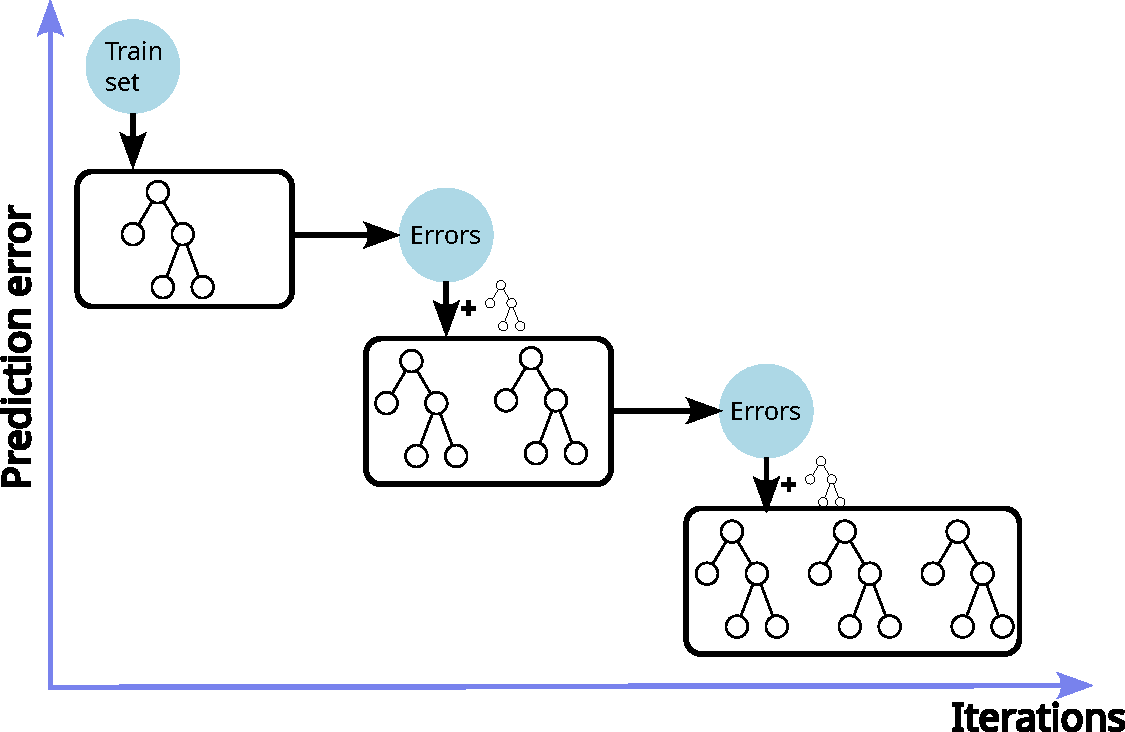
\includegraphics[width=\textwidth]{gradient_boosting}
\end{frame}

\begin{frame}[fragile]
  \frametitle{Gradient Boosting Hyperparameters}

  \begin{block}{Number of trees}
    Same as before : 
    \begin{itemize}
    \item low number : fast to compute, but less accurate
    \item high number : slower to compute, but more accurate up to some number
    \end{itemize}
  \end{block}

  \begin{block}{Tree depth}
    Specify the maximal depth of tree. An higher depth will make dedicate
    categories, but less generalizable.
  \end{block}
\end{frame}

  \begin{block}{Learning rate}
    Determine how much each weak learner contributes to the decision
    \begin{itemize}
    \item Regularization : small values produces a better test error
    \item help : \url{https://scikit-learn.org/stable/modules/ensemble.html#gradient-boosting-shrinkage}
    \end{itemize}
  \end{block}


  \begin{frame}[allowframebreaks,fragile]
    \frametitle{Implementations of Boosting}
    \begin{block}{GradientBoosting with sklearn}
      \begin{minted}
        [
          frame=lines,
          framesep=2mm,
          baselinestretch=1.2,
          fontsize=\footnotesize,
          linenos
        ]
        {python}
        from sklearn.ensemble import GradientBoostingClassifier
        n_estimators = 20 # the number of weak learners
        learning_rate = .1
        clf = GradientBoostingClassifier(n_estimators=n_estimators,
        learning_rate=learning_rate)
        clf.fit(X,y)
        ypred = clf.predict(X)
      \end{minted}

    \end{block}
    \framebreak
    \begin{block}{XgBoost}
      \begin{minted}
        [
          frame=lines,
          framesep=2mm,
          baselinestretch=1.2,
          fontsize=\footnotesize,
          linenos
        ]
        {python}
        import xgboost as xgb
        n_estimators = 20 # the number of weak learners
        learning_rate = .1
        clf = xgb.XGBClassifier(n_estimators=n_estimators,
        learning_rate=learning_rate)
        clf.fit(X,y)
        ypred = clf.predict(X)
      \end{minted}
    \end{block}
  \end{frame}

% =================================================================================
\section{Conclusion}
% =================================================================================

\begin{frame}{Conclusion}
  \begin{block}{Decision trees and Co.}
    \begin{itemize}
    \item Works (very) well on tabular data
    \item Interpretable
    \item State of the art on many challenges (Kaggles)
    \item Overfitting
    \item Need of a tabular representation of the data 
    \end{itemize}
    
  \end{block}
\end{frame}

% =================================================================================
\nocite{*}
\begin{frame}
  \frametitle{References}
    \begin{block}{References}
      \bibliographystyle{plainnat}
      \bibliography{biblio}
  \end{block}
\end{frame}



\end{document}
